\documentclass[11pt,a4paper,oneside]{article}
\usepackage[utf8]{inputenc}
\usepackage{a4wide}
\usepackage{url}
\usepackage{hyperref}

%\usepackage[chapter]{algorithm}
%\floatname{algorithm}{Alg.}
\usepackage{ifpdf}
\ifpdf
\usepackage[pdftex]{graphicx}
\DeclareGraphicsExtensions{.pdf,.png,.gif,.jpg}
\else
\usepackage[final]{graphicx}
\DeclareGraphicsExtensions{.eps,.png,.gif,.jpg}
\fi



\begin{document}


\centerline{{\Large Paralelní a distribuované algoritmy}}
\centerline{\Huge{Pipeline merge sort}}
\bigskip
\centerline{\large Svätopluk Hanzel \tiny (xhanze10)}
\centerline{\small \today}


\section{Algorithm description}
	\textit{Pipeline Merge sort} is a modification of merge sort, where several processors perform independent parts of the merging process. The main difference is that the processors do not have all the numbers available locally. They are connected in pipeline via 2 links (except the first and last processor) through which the numbers are gradually pumped along. Also not all processors merge sequences of the same length -- the further down a processor is, the longer the sequences it merges. \cite{akl2014parallel}
	
	For a sequence of numbers of length $n$ we will need $k = log_2 n$ processors. Each processor $P_i | i = 1..k$ sorts 2 subsequences of length $2^{i-1}$ into one subsequence of length $2^i$.
	
	\begin{figure}[h]
		\centering
		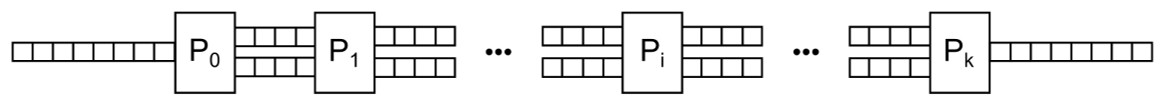
\includegraphics[width=0.7\linewidth]{img/pipeline.jpg}
		\caption{The pipeline}
		\label{fig:pipeline}
	\end{figure}

	\paragraph{First processor} $P_0$ is responsible for reading the initial sequence and sending it to the next processor while alternating the used link.
	\paragraph{Core processors} $P_1 \dots P_{k-1}$ first wait for the first link to have enough values ($2^{i-1}$) and the second link to have at least one value. It then starts merging these sequences by comparing the first values from both links and sending the lower onto the next processor ($P_i+i$). After sending a whole sequence of $2^i$ numbers it switches the link.
	\paragraph{Final processor} $P_k$ waits for links to be filled up and then starts the final merging of the sequence in similar way as the core processors.
	
	\subsection{Cost analysis}
		Processor $P_i$ starts sort when there is at least $2^{i-1}$ numbers on one link and at least one number on the other, which is $2^{i-1} + 1$ cycles after the previous processor $P_{i-1}$ has started. Therefore $P_i$ starts sorting in cycle
		\[
			1+\sum_{j=0}^{i-1}2^j + 1 = 2^i + i
		\]
		
		After processing all the remaining $n-1$ elements $P_i$ stops in cycle $(n-1) + 2^i + i$. The Final processor $P_k$ finishes in cycle
		\[
			2^k + k + (n-1) = 2^{log_2 n} + log_2 n + (n-1) = 2n + log_2 n - 1
		\]
		This algorithm has a running time $O(n)$ and space complexity $p(n) = log_2 n +1$, which gives us the overall cost
		\[
			c(n) = t(n) \times p(n) = O(n log_2 n)
		\]
	

\section{Implementation}
	This project is implemented in C++ using the \textit{OpenMPI} library. Main file is called \texttt{pms.cpp}, which contains the \texttt{main} function and is responsible for initializing the MPI library. The processors are implemented in \texttt{pms.h}. Each stage has its own class -- \texttt{Initializer}, \texttt{Middleman}, and \texttt{Finalizer}. All of these classes inherit the \texttt{Process} class which is responsible for providing process details and finalizing the MPI once the object ends its lifespan.
	
	The processes use MPI's \texttt{COMM\_WORLD} communicator and uses 2 tags - \texttt{MSG\_PIPELINE0} and \texttt{MSG\_PIPELINE1} to indicate which pipeline should be used on the receiver's end. After the message is received it is saved into a \texttt{std::queue} container for further processing.
	
	\begin{figure}[h]
		\centering
		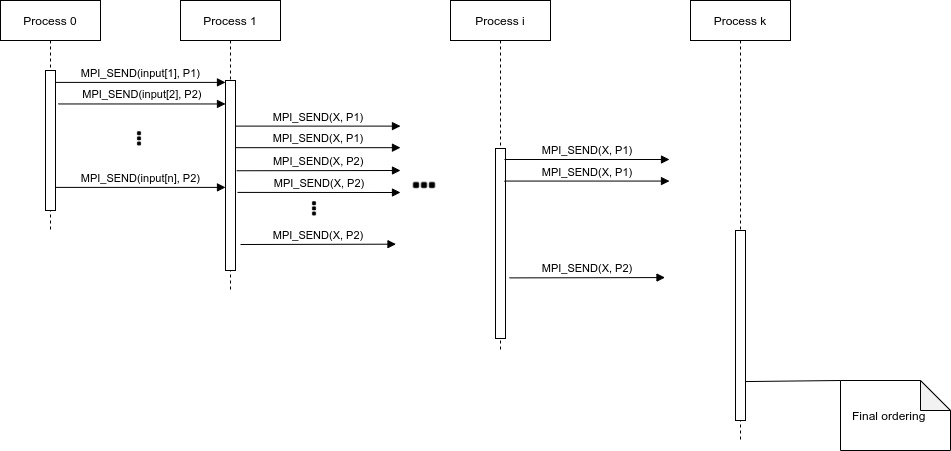
\includegraphics[width=1\linewidth]{img/diagram}
		\caption{Communication diagram}
		\label{fig:diagram}
	\end{figure}
	

\section{Conclusion}
	The project is fully finished and was tested and confirmed working in both local (development) and reference environment (merlin.fit.vutbr.cz).
	
\bibliographystyle{acm}
\bibliography{report}

\end{document}